% -----------------------------------------------------------------
% Document class: Article
\documentclass[ a4paper, twoside, 11pt]{article}
\usepackage{../../macros-general}
\usepackage{../../macros-article}
%\graphicspath{{./figures/}}
% Number of the handout, quiz, exam, etc.
\newcommand{\numero}{03}
\setcounter{numero}{\numero}

% -----------------------------------------------------------------
\begin{document}
\allowdisplaybreaks

% Indices
\newcommand{\iava}{$i$\tsup{ava} }
\newcommand{\iavo}{$i$\tsup{avo} }
\newcommand{\java}{$j$\tsup{ava} }
\newcommand{\javo}{$j$\tsup{avo} }
\newcommand{\kava}{$k$\tsup{ava} }
\newcommand{\kavo}{$k$\tsup{avo} }
\newcommand{\tava}{$t$\tsup{ava} }
\newcommand{\tavo}{$t$\tsup{avo} }
\newcommand{\tmava}{$(t-1)$\tsup{ava} }
\newcommand{\tmavo}{$(t-1)$\tsup{avo} }
\newcommand{\tMava}{$(t+1)$\tsup{ava} }
\newcommand{\tMavo}{$(t+1)$\tsup{avo} }

\begin{center}
\Large Modelos Estoc\'asticos (INDG-1008): Lecci\'on \numero \\[2ex]
\small \textbf{Semestre:} 2017-2018 T\'ermino II \qquad
\textbf{Instructor:} Luis I. Reyes Castro
\end{center}
\fullskip

% -----------------------------------------------------------------
\begin{problem}
El aeropuerto internacional de Centerville tiene dos pistas, una solo para despegues y otra solo para aterrizajes. Los aviones llegan al espacio a\'ereo del aeropuerto, el cual tiene una capacidad para $C = 7$ aeronaves, para pedir instrucciones de aterrizaje seg\'un un proceso de Poisson con tasa media de $\lambda$ por hora. El tiempo que se requiere para realizar un aterrizaje despu\'es de la aprobaci\'on tiene distribuci\'on exponencial con media de $\mu = 3$ minutos, proceso que debe estar terminado antes de aprobar otro aterrizaje. Los aviones en espera de pista vuelan en c\'irculos. 

La FAA (Administraci\'on de Aviaci\'on Federal, por sus siglas en ing\'es) tiene varios criterios respecto del nivel seguro de congesti\'on de aviones en espera para aterrizar. Estos criterios dependen de varios factores en cada aeropuerto, como el n\'umero de pistas disponibles. En el caso de Centerville los criterios son \textit{(i)} el n\'umero promedio de aviones en espera no debe exceder de 1, \textit{(ii)} el 95\% del tiempo, el n\'umero real de aviones en espera no debe exceder de 4, y \textit{(iii)} para el 99\% de los aviones, el tiempo que vuelan en c\'irculos antes de aterrizar no debe exceder de 30 minutos. 

Complete las siguientes actividades: 
\begin{enumerate}[label=\textbf{\alph*)}]
\item \textbf{2 Puntos:} Calcule la distribuci\'on estacionaria del sistema para los casos cuando la tasa de arribo es de $\lambda = 10$ por hora, $\lambda = 15$ por hora, y $\lambda = 25$ por hora. 
\item \textbf{2 Puntos:} Para cada uno de los tres casos anteriores, eval\'ue si se cumplen o no los requisitos de la FAA. 
\item \textbf{2 Puntos:} Suponga que se construye otra pista de aterrizaje. Recalcule la distribuci\'on estacionaria del sistema para los casos cuando la tasa de arribo es de $\lambda = 10$ por hora, $\lambda = 15$ por hora, y $\lambda = 25$ por hora. 
\item \textbf{2 Puntos:} Para cada uno de los tres casos anteriores, eval\'ue si se cumplen o no los requisitos de la FAA. 
\end{enumerate}

\end{problem}
\fullskip

% -----------------------------------------------------------------
\begin{problem}
\textbf{[8 Puntos]} El lunes, cierta acci\'on cerr\'o a 10 d\'olares. El martes se espera que la acci\'on cierre a 9, 10 u 11 d\'olares, con probabilidades respectivas de 0.3, 0.3 y 0.4. El mi\'ercoles, se espera que la acci\'on cierre 10\% abajo, sin cambio o 10\% arriba del cierre del martes, con las siguientes probabilidades: 

\begin{figure}[htb]
\centering
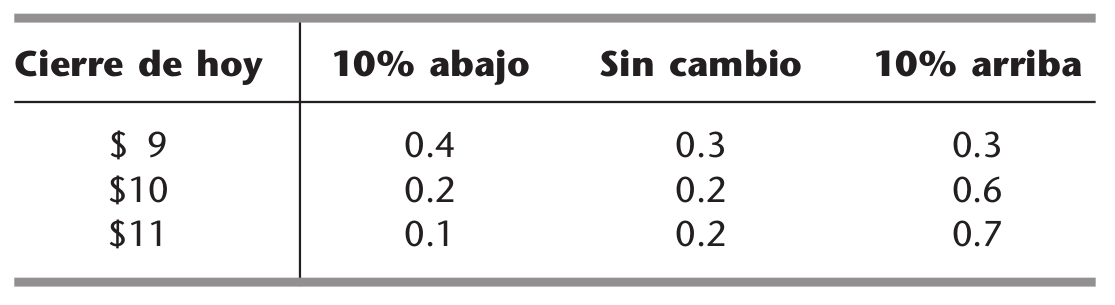
\includegraphics[width=0.6\textwidth]{problema-acciones.jpg}
\end{figure}

El martes recibe instrucciones de comprar 100 acciones antes del jueves. Todas las compras se hacen al final del d\'ia, al precio de cierre conocido de ese d\'ia, de manera que sus \'unicas opciones son comprar al final del martes o al final del mi\'ercoles. Usted quiere determinar una estrategia \'optima: comprar el martes o aplazar la compra hasta el mi\'ercoles, dado el precio al cierre del martes, con el fin de minimizar el precio esperado de compra. Desarrolle y eval\'ue un \'arbol de decisi\'on para determinar la estrategia \'optima. 
\end{problem}
\fullskip

\end{document}
